\documentclass[10pt,a4paper]{article}
\usepackage[T1]{fontenc}
\usepackage[utf8]{inputenc}
\usepackage{lmodern}
\usepackage{amsmath,amssymb}
\usepackage{booktabs}
\usepackage{tabularx}
\renewcommand{\tabularxcolumn}[1]{>{\raggedright\arraybackslash}p{#1}}
\usepackage{graphicx}
\usepackage[margin=2.2cm]{geometry}
\usepackage{microtype}
\usepackage[hidelinks]{hyperref}
\usepackage{float}
\setlength{\parskip}{4pt}
\setcounter{section}{1}
\title{A spiking descending layer for flapping-wing manoeuvres: method and results}
\author{}
\date{Draft, 2026-10-22}
\begin{document}
\maketitle

\noindent\emph{Draft of the Method and Results sections (no Introduction / Related work). Every number is traceable to \texttt{artifacts/spike\_steer/plan\_v*/} in the repository (branch \texttt{research/original-env-snn-neat}); method figures are \texttt{docs/paper/figs/fig\_m*.png}, results figures \texttt{docs/paper/figs/fig\_r*.png}.}


\section{Method}

\subsection{Platform and interface}

\textbf{Vehicle and simulator.} The vehicle is the IST\_robot-V2 flapping-wing micro air vehicle (15 g, one motor driving two wings at $\approx$26.7 Hz, i.e. a 37 ms wingbeat; IMU on the lower body). It is simulated in MuJoCo 3.8.0 as a multibody system with blade-element aerodynamics whose lift is calibrated against bench measurements of the real vehicle. The controller runs at 500 Hz (2 ms tick); the plant integrates at 200 kHz (400 physics sub-steps per tick).

\textbf{Interface (unchanged throughout).} At every tick the controller receives the 11-dimensional sensor vector \texttt{[roll, pitch, yaw (rad), gx, gy, gz (rad/s), ax, ay, az (m/s$^{2}$), z (m), vz (m/s)]}: attitude and rates from the IMU with Gaussian noise (0.02$^\circ$, 0.002 rad/s, 0.02 m/s$^{2}$), \texttt{z} from a time-of-flight range finder (50 Hz, 20 ms latency, 2 mm noise) and \texttt{vz} from an $\alpha$-$\beta$ observer. It commands the two gimbal angles $\alpha$, $\beta$ $\in$ $\pm$0.3 rad and the motor speed $\omega$ $\in$ [3115, 3807] rad/s; the commands are updated every 2 ms and pass through an 8.2 ms first-order actuator lag. Measured hover needs $\approx$3140 rad/s, only $\approx$25 rad/s above the lower limit, so downward thrust authority is small. The sensor set, actuator set, update rate and limits (\texttt{LOW}/\texttt{HIGH}, \texttt{DT}, the untouched \texttt{ControlEnv}) are shared by every controller in this paper; new test scenarios only change the case definitions (Section 2.6).

\textbf{Stress condition.} All training, validation and blind cases are "stress" cases: initial attitude error $\pm$5$^\circ$, motor gain uncertainty $\pm$1.5 \%, accelerometer bias 0.01 m/s$^{2}$ and attitude bias 0.05$^\circ$, one control step (2 ms) of sensor delay, and periodic disturbance pulses: a force of 0.006 N and a torque of 8$\cdot$10$^{-6}$ N$\cdot$m, switched on for 0.2 s whenever \texttt{t mod 2 s $\in$ [0.6, 0.8) s} (i.e. at 0.6, 2.6 and 4.6 s) with a random sign per episode, so one pulse lands 0.2--0.4 s into every redirect and dash manoeuvre. Each case is one random seed; eight strata fix the wing state at release (the wingbeat phase at take-off). Episodes last 5 s (evade) or 6.5 s (redirect, dash).

\subsection{Manoeuvre tasks and scoring}

Three manoeuvres are commanded during hover (Fig. M5, \texttt{fig\_m5\_tasks.png}). Directions are given in the heading frame fixed at the command onset \texttt{t0} (yaw at \texttt{t0}; 0$^\circ$ = forward, 90$^\circ$ = left); the measured attitude-to-motion sign map is (roll, pitch)\_ref $\propto$ ($-$sin $\varphi$, +cos $\varphi$). The command is a unit vector (cos $\varphi$, sin $\varphi$) on one of two channels (evade; dash/redirect) and is presented to the learned layer as eight rectified inputs ($\pm$ of each component on each channel). The command switches off when the goal is detected on the ground-truth position.

\begin{table}[htbp]\centering\scriptsize
\begin{tabularx}{\textwidth}{lXXlX}\toprule
task & command & goal & window & classes \\ \midrule
\textbf{evade} & displace 0.10 m along $\varphi$ $\in$ \{0, 90, 180, 270\}$^\circ$; \texttt{t0 \textasciitilde{} U(2.2, 2.8) s} & reach 0.10 m as fast as possible & 1.5 s & pitch (0/180$^\circ$), roll (90/270$^\circ$) \\
\textbf{redirect} & go along $\varphi_1$ $\in$ \{0, 90, 180, 270\}$^\circ$; when 0.08 m or 1.0 s is reached the command switches to $\varphi_2$ = $\varphi_1$ $\pm$ 90$^\circ$; \texttt{t0 = 2.4 s} & reach 0.10 m along $\varphi_2$ after the switch with little overrun along $\varphi_1$ & 4 s & by $\varphi_2$: pitch, roll \\
\textbf{dash} & displace 0.15 m along $\varphi$ $\in$ \{0, 45, \ldots{}, 315\}$^\circ$ and stop; \texttt{t0 = 2.4 s} & reach, then settle (speed along $\varphi$ < 0.1 m/s for 0.3 s), little overshoot & 4 s & pitch, roll, diagonal \\
\bottomrule\end{tabularx}\end{table}

\textbf{Score (lower is better).} With \texttt{W} the window, \texttt{short} the shortfall to the goal distance (m), \texttt{cross} the lateral position error at the reach time (evade) or at the end of the window (dash), \texttt{max|$\Delta$z|} the largest altitude deviation (cm) from the altitude at \texttt{t0} over the rest of the flight (symmetric; plan v9 onwards), and \texttt{crash = 10 + 5$\cdot$(unflown fraction of the window)} if the episode terminated early (else 0):

\begin{itemize}\setlength\itemsep{2pt}
\item evade: \texttt{(t\_reach, or 1.5 + 10$\cdot$short) + 0.5$\cdot$|cross| + 0.03$\cdot$max|$\Delta$z| + crash};
\item redirect: \texttt{t\_switch + (t\_reach2, or (4 $-$ t\_switch) + 10$\cdot$short) + 2$\cdot$max(0, overrun $-$ 0.05) + 0.03$\cdot$max|$\Delta$z| + crash}, where \texttt{overrun} is the displacement along $\varphi_1$ after the switch; a case that never switches scores \texttt{4 + 10$\cdot$0.10 + \ldots{}};
\item dash: \texttt{(t\_reach, or 4 + 2$\cdot$short) + (t\_settle, or 4) + 2$\cdot$max(0, max\_along $-$ 0.25) + 0.5$\cdot$|cross| + 0.03$\cdot$max|$\Delta$z| + crash}.
\end{itemize}

A \textbf{crash} is any early termination: true tilt > 80.2$^\circ$, |z $-$ z\_start| > 1 m, absolute height z < 0.12 m, any body part within 3 cm of the ground, or a numerical failure. Tilt is the true angle between the body axis and the vertical (acos R$_{33}$ from the simulator state).

\textbf{Ratio.} For comparability across tasks and directions, each case score is divided by the median score of the classical opponent over the blind cases of the same direction class (32 cases per class for evade and redirect; 16/16/32 for dash pitch/roll/diagonal); the task ratio is the mean over cases and the \emph{manoeuvre ratio} is the mean over the three tasks. Because the score distributions are right-skewed, this ratio is above 1 even for the opponent itself (1.089 on the plan-v11 blind set, Section 3.1). The main comparisons therefore use the \textbf{paired difference} $\Delta$ = (arm ratio $-$ opponent's own ratio) on identical cases, with a paired bootstrap 95 \% interval over cases within task (4000 resamples), the paired win count, and crash counts with exact Clopper--Pearson 95 \% intervals.

\subsection{Hierarchical controller}

The controller has three layers (Fig. M1, \texttt{fig\_m1\_architecture.png}; one 2 ms tick in Fig. M3, \texttt{fig\_m3\_gating.png}).

\textbf{Reflex layer --- PID.} A PID attitude loop drives the gimbal: \texttt{e = ref $-$ [roll, pitch]}, derivative on the measurement through a 4.5 ms low-pass, integral clipped to $\pm$0.3 with anti-windup, \texttt{[$\alpha$, $\beta$] = trim + [effort\_pitch, effort\_roll]}; a PID altitude loop sets the motor speed (gains 900, 500, 80 on z error, vz and $\int$z). The attitude gains were re-tuned on stress hover (kp $\times$ 1.5, kd $\times$ 0.85, ki $\times$ 1.5 relative to the original baseline); a full-state-feedback upper bound improves the hover tilt RMS by only 1.1$^\circ$, so no learned component touches hovering.

\textbf{Steering-muscle layer --- phase-locked motor pulses.} A motor pulse drives the motor command to its maximum (3807 rad/s) for a few milliseconds; after the 8.2 ms actuator lag it raises the speed by $\approx$690 rad/s during part of a wingbeat, and the resulting lift asymmetry within the stroke produces a \textbf{pitch torque} whose sign depends on the wingbeat phase of the pulse. The classical pulse law (the base law of every arm, active outside manoeuvre commands) is \texttt{u = $-$(k\_$\theta\cdot$pitch + k\_q$\cdot$q\_slow)} with k\_$\theta$ = 8.0, k\_q = 0.4, \texttt{q\_slow} the pitch rate with the wingbeat harmonics notched out, and a PLL estimate of the crank phase; it holds the maximum command while \texttt{|u| > 0.5} and the phase is within $\pm$22.5$^\circ$ of 135$^\circ$ (u > 0) or 315$^\circ$ (u < 0), i.e. $\approx$4.6 ms per wingbeat at most. The learned layer's pulses are 3-tick (6 ms) twitches triggered by output spikes (next paragraph).

\textbf{Descending layer --- the spiking network} (Fig. M2, \texttt{fig\_m2\_snn.png}). A leaky integrate-and-fire (LIF) network with axonal delays:

\begin{itemize}\setlength\itemsep{2pt}
\item input \texttt{x\_t $\in$ $\mathbb{R}^{25}$} per tick: eight IMU channels (roll, pitch, gx, gy, gz, ax, ay, az) scaled by 0.1 rad, 10 rad/s and 25 m/s$^{2}$ respectively and split into rectified + and $-$ channels (16), a constant 1 (bias), and the eight rectified command channels;
\item 11 input delay taps \texttt{k = 0\ldots{}10} ticks (0--20 ms): hidden drive \texttt{I\_h(t) = $\sum$\_k W\_in[:, :, k] x\_\{t$-$k\} + b\_h}, \texttt{W\_in $\in$ $\mathbb{R}$\^{}\{8$\times$25$\times$11\}};
\item 8 hidden LIF neurons updated in two 1 ms sub-steps per tick as unit-gain first-order filters, \texttt{c $\leftarrow$ a\_s c + (1 $-$ a\_s) I}, \texttt{v $\leftarrow$ a\_m v + (1 $-$ a\_m) c}, \texttt{a = exp($-$1 ms / $\tau$)}, spike when \texttt{v $\ge$ 1} followed by subtractive reset; $\tau$\_m and $\tau$\_s are learned in the imitation stage and frozen afterwards (selected centres: $\tau$\_m = 1.9--2.1 ms, $\tau$\_s = 1.05--1.15 ms);
\item hidden $\rightarrow$ output through 11 axonal delays \texttt{d = 0, 2, \ldots{}, 20 ms} on the hidden spike trains \texttt{s}, with a fixed spike scale of 5: \texttt{I\_o = 5$\cdot\sum$\_d W\_out[:, :, d] s\_\{t$-$d\} + b\_o} into two output LIF neurons of the same form (\texttt{b\_o} initialised to $-$2), and \texttt{I\_g = 5$\cdot\sum$\_d W\_g[:, :, d] s\_\{t$-$d\} + b\_g} into two graded units \texttt{g $\leftarrow$ a\_g g + (1 $-$ a\_g) c\_g}, $\tau$\_g = 20 ms;
\item outputs: a spike of either output neuron triggers one 3-tick motor twitch (two output neurons are two routes to the same twitch; the timing within the wingbeat carries the meaning); the graded units give the \textbf{roll and pitch set-points} \texttt{ref = 0.7 rad $\cdot$ tanh(g)} handed to the PID;
\item 2564 parameters in total (\texttt{W\_in}, \texttt{b\_h}, \texttt{W\_out}, \texttt{b\_o}, \texttt{W\_g}, \texttt{b\_g}); the network has no notion of height or of time since the command (plan v10 tested 12 extra inputs for these and found no gain).
\end{itemize}

\textbf{Command gate and safety rules.} The learned layer is in charge only while a command is on and for a 1 s tail after it ends; outside the gate the base pulse law acts and the set-points are zero, so every arm flies identically tick for tick before \texttt{t0} (checked bit-exactly: the prefix cache of Section 2.4 reproduces the plain episode to the last bit, and in the pre-command-hit scenario of Section 3.3 all arms had identical pre-\texttt{t0} traces on 192/192 cases). While in charge: pulse onsets are separated by a refractory period of at least 37 ms, and the righting reflex is off. Outside the gate, if the sensed tilt exceeds 25$^\circ$ the base law is replaced for the rest of the episode by a righting pulse law (k\_$\theta$ = 3.0, k\_q = 0.4, threshold 0.5, 90$^\circ$ window). The learned layer can act no earlier than 1.5 s after take-off (before that its set-points are zeroed and its pulses suppressed).

\subsection{Training}

The pipeline (Fig. M4, \texttt{fig\_m4\_pipeline.png}) has three stages; the controller that is tested is the frozen output of stage 3. All stages run in the stress condition on disjoint seed ranges (training, validation and blind sets never share a seed).

\textbf{Stage 1 --- imitation of the classical schedule.} The classical opponent (Section 2.5) flies 16 training and 4 validation cases per task. From \texttt{t = 2 s} on, every tick records the 25-D input, whether the opponent fired a pulse (its base-law pulses are suppressed while a schedule segment is active, so the teacher fires only outside active segments), the sign of its law variable \texttt{u} (the nose-up / nose-down label), and its set-points. A torch twin of the network with identical tick arithmetic is trained by back-propagation through time with a sigmoid surrogate gradient (slope 1/0.25) on windows of 200 ticks (stride 100, batches of 32 windows). The loss is \texttt{mean[(1 + 2y)$\cdot$BCE(p, y)] + 5$\cdot$mean[(ref/0.7 $-$ r)$^{2}$]}, where \texttt{y} is the recorded pulse label, \texttt{p = max over the two sub-steps of $\sigma$((v\_o $-$ 1)/0.25)} is the surrogate firing probability of the output neuron of the labelled sign, and \texttt{r} the recorded set-points; Adam 3$\cdot$10$^{-3}$, gradient norm clipped to 1, 40 epochs, best epoch by validation loss. Five seeds give five imitation starts, shared by all plans from v7 on.

\textbf{Stage 2 --- OpenAI-ES on the manoeuvre score.} Starting from the imitation weights $\theta_{0}$ (the six weight/bias tensors; the time constants are frozen), each generation draws 8 antithetic pairs (population 16) of perturbations $\varepsilon$ \textasciitilde{} N(0, I), evaluates $\theta$ + $\sigma\varepsilon$ and the centre $\theta$ on the generation's batch, and updates $\theta$ with rank-based utilities (\texttt{u\_i $\propto$ max(0, log(9) $-$ log(rank\_i + 1))}, centred), the gradient estimate \texttt{$\sum$ u\_i $\varepsilon$\_i / $\sigma$} normalised by Adam moments (0.9, 0.999, bias-corrected), $\sigma$ = 0.02, learning rate 0.01 $\cdot$ 0.85\^{}g, 16 generations (random seed 1000 + seed). The objective of a candidate is the mean over tasks of the mean over its cases of \texttt{score / N\_\{task,class\}}, where \texttt{N} is the opponent's class mean on 24 fixed normalisation cases per task, plus a soft tilt penalty of 0.3 per degree of the tilt peak above 60$^\circ$. Two features distinguish the final protocol (plan v11) from the earlier runs (plans v7--v10):

\begin{itemize}\setlength\itemsep{2pt}
\item \emph{full coverage}: 8 cases per task per generation, which covers all 8 dash directions, all 8 redirect pairs (both turn directions), all 4 evade directions and all 8 release strata every generation (the earlier 4-case batches used fixed direction slots --- dash 0/45/90/135$^\circ$ and one turn direction only --- and only strata 0--3, a defect found in plan v10);
\item \emph{crash-aware ranking}: any candidate with a crashed episode ranks below every crash-free candidate.
\end{itemize}

A generation costs 17 $\times$ 24 = 408 episodes (6 528 per seed). The population shares the pre-command prefix of each case through a bit-exact environment snapshot (\texttt{cache8}: a deep copy of the simulator state with the network state rebuilt by replaying the recorded inputs; verified to reproduce the plain episode bit for bit), so only the post-command part is simulated per candidate.

\textbf{Stage 3 --- selection.} The imitation start and the centre of every odd generation (9 centres) fly a fixed validation set of 64 cases per task (192 cases); centres with any crash or a tilt peak $\ge$ 70$^\circ$ are excluded and the centre with the lowest objective is selected. The selected centre is frozen; it is the only network that is ever evaluated on a blind set.

\subsection{Classical opponent and same-budget re-optimised schedule}

\textbf{Opponent.} The strongest classical scheme with the same actuators, PID and base law: an open-loop 2-D set-point schedule per task and direction class --- go set-point magnitude along $\varphi$, go duration, brake set-point magnitude (reversed) and brake duration, durations in 40 ms beats --- started by the command, restarted on a direction change (redirect) and ended by the command drop; base-law pulses are suppressed while a segment is active. Each schedule was tuned on its own grid and tuning cases (evade and redirect: 24 configurations $\times$ 8 cases per task; dash: 108 configurations $\times$ 16 cases, inherited from plan v6), best configuration per class by mean score. No learned component is involved. The opponent also provides the class medians of the ratio and the normalisers of the ES objective.

\textbf{Pulse suppression.} The opponent, as preregistered, suppresses its base-law pulses while a schedule segment is active (\texttt{pulse and not active}): the classical manoeuvre design is a PID with open-loop set-point schedules, and pulses --- the spike-timed channel of the learned layer --- are not part of it. A mechanism probe that gives the opponent its own hover pulse law back during the segments (\texttt{ClassicalUnsuppressed}; one changed line, no re-tuning) is described in Section 3.3; it was run after all other results were known (plan v14, preregistered on three sets and extended to the others by amendment) and is not a comparator of any criterion.

\textbf{Same-budget re-optimised schedule --- classical + ES (plan v11, amendment 1).} To test whether the score leaves room above the opponent at all, the 28 schedule parameters (7 classes $\times$ 4) were optimised with exactly the ES budget of stage 2 --- population 16, 16 generations, the same 24-episode batches with full coverage, crash-aware ranking --- with $\sigma$ = 0.05 and learning rate 0.02 in normalised parameter units (set-points divided by 0.5 rad, beat counts by 20), selected on the same 192 validation cases; four seeds on three machines. It bounds what the classical schedule family reaches with the learned layer's training budget.

\subsection{Evaluation protocol}

Every plan was preregistered: tasks, scoring, arms, blind-set seed base, number of cases and the pass criterion were committed to the repository before any blind episode (e.g. plan v11: commit \texttt{47d79a0}, before its first training episode; plan v12: \texttt{0726527}; plan v13 amendment 2: \texttt{abb78bc}), and amendments were committed before the episodes they cover; the one post-hoc amendment (\texttt{plan\_v12/amendment\_2\_post\_hoc.json}) demotes the plant-mismatch scenario from a primary to a secondary claim after its result was seen and is reported as such. Blind sets use seed bases never used before; each has 64 cases per task (192 episodes per arm) with the same direction and stratum coverage as the validation set. The classical opponent flies every blind case, so every comparison is paired. The reference machine (CloudPC-2, 32 vCPU) and a second machine (HomePC) produce identical episodes (0 differences in score, pulses and duration over 192 opponent episodes); a third machine (GoogleCloud) does not reproduce the reference bit for bit (floating-point differences amplified by the dynamics) and was used only for exploratory seeds that are reported separately, archived under \texttt{artifacts/spike\_steer/googlecloud/}, and never counted in a criterion.

\textbf{Robustness scenarios (plans v12--v13; frozen controllers, no training).} The selected v11 centres (5 seeds), the v9 centres (5 seeds), the imitation start of seed 1, the opponent and the two classical + ES centres were flown, unchanged, on fresh blind sets in which one element of the case is changed (Table R1 in Section 3):

\begin{itemize}\setlength\itemsep{2pt}
\item a 20 ms torque hit about a horizontal axis fixed in the heading frame (an external torque added to the body in the simulator), at a random time during the manoeuvre (\texttt{t0 + U(0.15, 0.45) s}; also early \texttt{+0--0.15 s}, late \texttt{+0.5--1.0 s}, before the command \texttt{$-$0.6\ldots{}$-$0.3 s}, a double hit 80--200 ms apart, and hits restricted to the roll or the pitch axis); magnitudes 2, 3 and 4.5 mN$\cdot$m, where 3 mN$\cdot$m was fixed before any learned-arm episode as the largest level at which the opponent crashes on $\le$ 20 \% of 24 calibration cases;
\item the periodic disturbance pulses of the stress condition scaled $\times$1.25 and $\times$1.5 ($\times$2 and $\times$3 were also run and lie beyond what any controller survives: all arms crash on nearly every case);
\item sensor degradation: attitude and gyro noise $\times$5 (0.10$^\circ$, 0.010 rad/s); sensor delay 3 steps (6 ms) instead of 1;
\item plant mismatch: lower-body mass and inertia +12.5 \% (a pre-existing out-of-distribution condition of the environment).
\end{itemize}

The preregistered criterion per scenario (H1) is: a v11 seed passes when its paired-$\Delta$ interval lies below 0 and its crashes do not exceed the opponent's; the scenario "holds" when $\ge$ 3 of 5 seeds pass. The 3 mN$\cdot$m mid-manoeuvre hit is the primary (confirmatory) scenario, formulated after the nominal criteria had failed and calibrated on the opponent only; the other scenarios were added by amendments before they ran and are reported descriptively with the same rule, without correction for multiplicity (17 blind sets were flown; 15 descriptive ones besides the primary scenario and its replication, each with 5 seeds). "Wins" counts cases with a strictly lower score than the opponent. The primary scenario was replicated once on a fresh seed base (plan v14). Plan v14 also added, after a review of this draft and before running: channel ablations of the frozen v11 centres under the primary hit (pulses suppressed while in charge; set-points zeroed while in charge); the imitation starts of seeds 2--5 under the primary hit and the $\times$1.5 disturbance; and the classical pulse-channel probe of Section 3.3.


\section{Results}

Two classical references appear throughout and are named consistently: the \textbf{classical opponent} (PID + hand-tuned open-loop set-point schedules; no pulses while a manoeuvre segment is active; the imitation teacher, the ES normaliser, the comparator of every criterion and the normaliser of every ratio) and \textbf{classical + ES} (the same schedules re-optimised with the ES budget, Section 2.5). Unless stated otherwise, $\Delta$ is the paired difference to the classical opponent on identical cases and crashes are counts out of 192. Three normalisations occur: the ES batch objective (class \emph{means} of the opponent on 24 fixed cases, plus the tilt penalty), the selection objective (the same normaliser on the 192 validation cases) and the blind ratio (class \emph{medians} of the opponent on the blind cases); they differ by 0.03--0.05 and are not interchangeable.

\subsection{Nominal manoeuvres}

\textbf{The preregistered ratio criterion was not met by any controller we trained.} Plans v7--v11 each asked, per seed, for a manoeuvre ratio $\le$ 0.95 with no more crashes than the opponent, in at least 3 of 5 seeds (Fig. R0). Plan v11, the final protocol, gives 1.046 / 1.146 / 1.033 / 1.054 / 1.063 for seeds 1--5 (Table R0) with \textbf{0 crashes in 960 blind episodes}; the earlier plans gave 0.97--1.07 with 10 crashes (opponent 5; plan v8, the v7 controllers re-tested on 64 cases per task), 1.02--1.13 with 3 crashes (opponent 0; v9) and 1.02--1.25 with 6 crashes (opponent 3; v10). The v7 "full" values of 0.89--1.00 (2 crashes, opponent 1) were obtained on 32 cases per task on a blind set where the opponent's own ratio was 1.18; re-tested on 64 fresh cases the same five controllers scored 0.97--1.07.

The ratio is above 1 for the opponent itself --- 1.089 on the v11 blind set, 1.086 on v9, 1.273 on v10, 1.415 on v8 --- because the per-case ratios are right-skewed (Fig. R0b: medians near 1, a tail of slow or crashed cases up to 3). Classical + ES reaches 1.019 / 1.032 on the bit-identical machines (0.999 / 1.018 on the approximate one) with 0 crashes and does not reach 0.95 either. An AI-assisted re-analysis of the per-case rows of plans v7--v10 (\texttt{plan\_v11/audit/audit\_report.md}, done before the v11 results) bounds the metric at 0.87--0.89 even when the best of the 5--14 available controllers is taken case by case, and in the dash task no controller met the settle condition in a single pitch- or diagonal-class episode (0 of $\approx$1 800 in v9--v10; 0 of all v11 episodes for all arms), so a constant 4 s term enters both numerator and denominator of that cell.


\begin{table}[htbp]\centering\scriptsize
\caption{Table R0 --- plan v11 blind set (base 2 099 100 000, 64 cases per task; opponent 0 crashes).}
\begin{tabularx}{\textwidth}{XXXXXXl}\toprule
arm & seed & machine & mean ratio & paired $\Delta$ to the opponent [95 \% CI] & wins /192 & crashes \\ \midrule
classical opponent (own ratio) & -- & CloudPC-2 & 1.089 & 0 & -- & 0 \\
classical + ES & 1 / 2 & CloudPC-2 / HomePC & 1.019 / 1.032 & $-$0.070 [$-$0.118, $-$0.029] / $-$0.056 [$-$0.100, $-$0.017] & 111 / 115 & 0 / 0 \\
SNN + ES & 1 & CloudPC-2 & 1.046 & $-$0.043 [$-$0.091, +0.001] & 100 & 0 \\
SNN + ES & 2 (= imitation start, see text) & CloudPC-2 & 1.146 & +0.057 [+0.015, +0.096] & 70 & 0 \\
SNN + ES & 3 & CloudPC-2 & 1.033 & $-$0.056 [$-$0.108, $-$0.008] & 110 & 0 \\
SNN + ES & 4 & HomePC & 1.054 & $-$0.035 [$-$0.092, +0.018] & 116 & 0 \\
SNN + ES & 5 & HomePC & 1.063 & $-$0.026 [$-$0.079, +0.024] & 116 & 0 \\
SNN, imitation only & 1 / 3 / 4 / 5 & -- & 1.166 / 1.137 / 1.238 / 1.257 & +0.077 / +0.049 / +0.149 / +0.168 & 46 / 63 / 55 / 42 & 0 \\
MLP + PPO reference & 1--5 & CloudPC-2 (HomePC policies) & 1.097 / 1.125 / 1.122 / 1.144 / 1.135 & +0.008 / +0.037 / +0.033 / +0.056 / +0.047 & 85 / 45 / 55 / 60 / 53 & 0 / 0 / 0 / 0 / 0 \\
\bottomrule\end{tabularx}\end{table}

\textbf{Parity with the classical opponent; 0.02--0.05 behind classical + ES.} Four of the five v11 seeds are at or slightly below the opponent ($\Delta$ $-$0.03 \ldots{} $-$0.06, one interval excluding 0); seed 2 is worse because its selection returned the imitation start (every ES centre of that seed crashed on the validation set). Paired directly against classical + ES (seed 1) the SNN seeds are +0.029 [+0.00, +0.05], +0.130, +0.017 [$-$0.02, +0.05], +0.039 [$-$0.00, +0.08] and +0.048 [+0.01, +0.08], i.e. 0.02--0.05 behind, two intervals including 0. ES improves four of the five seeds over their imitation starts by 0.10--0.19. Five exploratory seeds trained on the approximate machine behaved the same way (0.997--1.093, 0 crashes, every seed better than its start; rows in \texttt{artifacts/spike\_steer/googlecloud/}). Within tasks the four ES seeds are at or ahead of the opponent on evade and redirect (per-task $\Delta$ $-$0.02 \ldots{} 0.00 and $-$0.12 \ldots{} $-$0.19) and behind on dash (+0.02 \ldots{} +0.10); the dash roll class (90$^\circ$/270$^\circ$) is the weakest cell in every plan (v11: 1.17 / 1.00 / 1.40 / 1.56 / 1.52 by seed) and dash pitch the best (0.88--0.91 for the four ES seeds). In the roll class the learned layer reaches the target 13--29 \% sooner (0.44--0.54 s vs 0.617 s) but overshoots more (mean displacement beyond the 0.25 m penalty threshold 0.10--0.20 m vs 0.04 m) and, for seeds 3--5, settles later (0.99--1.36 s vs 0.58 s; seeds 1--2 0.46--0.58 s).

\textbf{Training and selection (Fig. R1).} Under the v11 protocol the ES centre objective on its 24-case batch falls from 1.05--1.16 to 0.92--0.96 (best per seed at generations 7--15); the SNN centre crashed on one batch case three times in 80 centre evaluations and the classical + ES centre once in 32 (seed 1, generation 14, objective 1.30), while 0--12 of the 16 perturbed candidates crash per generation and are ranked last. On the 192 validation cases the objective of the saved centres falls to 0.98--1.00 by generation 11--15 for seeds 3--5 (seed 5 rises again after generation 11 with crashes), seed 1 is best at generation 13 and seed 2 admits no ES centre; in plans v7--v10 every seed began to crash on the validation set after 2--10 generations. The classical + ES arm follows the same trajectory (batch objective 0.95--1.07 apart from that generation, validation 0.975), which locates the plateau in the task and score rather than in the learned layer. For reference, the five frozen MLP + PPO policies trained on the same tasks (plan v7 full, HomePC; three of them selected their imitation start) score 1.097--1.144 on the v11 blind set (Table R0; paired $\Delta$ +0.008 \ldots{} +0.056, 0 of 5 intervals below 0; 0 crashes in 960 episodes), i.e. the same parity band as the SNN; on the v8 blind set they scored 1.109 $\pm$ 0.024 with 1 crash where the SNN + ES centres scored 0.97--1.07 with 10 crashes.

\subsection{Robustness under disturbances}

All controllers are frozen and every arm flies the same cases. Table R1 gives the crash counts and the number of v11 seeds passing H1; Fig. R2 shows the rates and Fig. R3 the paired $\Delta$ of every seed. Only the 3 mN$\cdot$m mid-manoeuvre hit (and its replication) is confirmatory; the other rows are descriptive, uncorrected for multiplicity (17 blind sets flown; 15 descriptive ones besides the primary scenario and its replication, each with 5 seeds), and H1 is degenerate where the opponent does not crash (mass +12.5 \%, roll-axis hit) or where every arm crashes ($\times$2, $\times$3 disturbance: the rule passes formally at $\times$2 with 174 vs 192 crashes and is not counted).


\begin{table}[htbp]\centering\scriptsize
\caption{Table R1 --- crashes /192 on the blind robustness sets. The v9 centres, the imitation starts, the opponent's own ratio and the per-seed $\Delta$ with intervals are in the per-scenario \texttt{summary\_*.json} files of plans v12--v13, in \texttt{plan\_v14/crash\_table\_with\_unsuppressed.md} and in \texttt{docs/paper/data/robustness\_crashes.csv}. Seed 2 of SNN + ES is its imitation start. $\star$: rows in which the imitation starts of all five seeds were also flown (reported in the text).}
\begin{tabularx}{\textwidth}{XlXXX}\toprule
scenario & opponent & classical + ES s1 / s2 & SNN + ES v11, seeds 1--5 & v11 seeds passing H1 (of 5) \\ \midrule
hit 2 mN$\cdot$m, +0.15--0.45 s & 17 & 16 / 16 & 9 / 4 / 8 / 2 / 6 & 5 \\
\textbf{hit 3 mN$\cdot$m, +0.15--0.45 s (primary)} $\star$ & 60 & 56 / 58 & 40 / 32 / 34 / 22 / 40 & \textbf{4} \\
\textbf{same, replication, fresh base} & 42 & 41 / 43 & 39 / 23 / 21 / 16 / 31 & \textbf{4} \\
hit 4.5 mN$\cdot$m & 86 & 87 / 89 & 95 / 71 / 67 / 46 / 76 & 1 \\
hit 3 mN$\cdot$m, +0--0.15 s & 56 & 53 / 56 & 42 / 30 / 31 / 22 / 45 & 4 \\
hit 3 mN$\cdot$m, +0.5--1.0 s & 40 & 39 / 33 & 12 / 5 / 14 / 9 / 16 & 5 \\
hit 3 mN$\cdot$m, 0.3--0.6 s before the command & 7 & 3 / 6 & 4 / 2 / 1 / 1 / 2 & 3 \\
double hit 3 + 3 mN$\cdot$m & 84 & 86 / 80 & 73 / 69 / 60 / 44 / 68 & 2 \\
hit about the roll axis only & 0 & 2 / 0 & 17 / 0 / 0 / 0 / 0 & 4 (degenerate) \\
hit about the pitch axis only & 74 & 71 / 71 & 46 / 48 / 47 / 36 / 51 & 3 \\
disturbance pulses $\times$1.25 & 10 & 5 / 8 & 2 / 0 / 1 / 2 / 0 & 5 \\
disturbance pulses $\times$1.5 $\star$ & 40 & 36 / 38 & 7 / 5 / 9 / 8 / 9 & 5 \\
disturbance pulses $\times$2 / $\times$3 & 192 / 192 & 192 / 192 & 174--175 / 192 & not counted \\
IMU noise $\times$5 & 3 & 1 / 1 & 3 / 0 / 1 / 1 / 1 & 1 \\
sensor delay 3 steps & 9 & 11 / 12 & 2 / 0 / 4 / 4 / 4 & 4 \\
mass +12.5 \% (secondary) & 0 & 0 / 0 & 0 / 0 / 0 / 0 / 0 & 0 (degenerate) \\
\bottomrule\end{tabularx}\end{table}

\textbf{Primary scenario and its replication.} With a 3 mN$\cdot$m hit landing 0.15--0.45 s into the manoeuvre the opponent crashes in 60 of 192 cases, classical + ES in 56--58, the v11 SNN centres in 22--40 and the imitation starts in 23--32. The paired $\Delta$ of the five seeds is $-$0.125 [$-$0.426, +0.209], $-$0.282 [$-$0.448, $-$0.121], $-$0.355 [$-$0.540, $-$0.186], $-$0.584 [$-$0.815, $-$0.377] and $-$0.263 [$-$0.473, $-$0.024]: \textbf{H1 holds (4 of 5)}. On a fresh seed base the result replicates (42 vs 16--39 crashes; $\Delta$ $-$0.09 \ldots{} $-$1.05; 4 of 5, seed 1 failing both times). Per task, the gain is in dash (2--10 crashes vs 19) and redirect (12--22 vs 24); evade crashes less too (6--13 vs 17) but its $\Delta$ has no consistent sign. The MLP + PPO reference, which has the same set-point authority but no pulse channel, crashes 41--47 times on the same cases ($\Delta$ -0.207 \ldots{} -0.113).

\textbf{Dose--response, timing, axis, repetition (Fig. R4).} At 2 mN$\cdot$m the SNN crashes 2--9 times against 17 ($\Delta$ $-$0.57 \ldots{} $-$0.89, all seeds); at 4.5 mN$\cdot$m the opponent crashes in 45 \% of the cases, the SNN in 24--49 \%, and only seed 4 remains significantly better ($\Delta$ $-$0.65 [$-$0.94, $-$0.40]; seed 1 is worse, +0.40 [+0.00, +0.79]). The advantage shrinks once the hit exceeds what the learned layer's own tilt margin (the distance from its operating tilt to the 80$^\circ$ crash threshold) can absorb, as anticipated, with a hedge, in the amendment. The amendment on hit timing expected the largest advantage for early hits; the opposite was found: late hits (0.5--1.0 s, during braking and settling, with the learned layer still in charge through its 1 s tail) give 5--16 crashes against 40, all seeds passing, whereas early hits (0--0.15 s, during the initial lean) are the hardest for everyone (56 vs 22--45). A hit 0.3--0.6 s before the command produces bit-identical trajectories up to \texttt{t0} for all arms (192/192 cases; checked by comparing, per case, the number of pre-\texttt{t0} ticks and the sums of the attitude, position and velocity columns of the trace), after which the learned layer handles the command arriving during recovery with 1--4 crashes against 7. Hits about the roll axis crash the opponent 0 times and the other arms 0--2 times, except v11 seed 1 (17 crashes; $\Delta$ +0.84 [+0.42, +1.32]), so this scenario cannot separate the arms; hits about the pitch axis crash the opponent in 74 cases and the SNN in 36--51, in line with the random-axis result. A second hit 80--200 ms after the first reduces the margin again (84 vs 44--73, 2 of 5).

\textbf{Sustained disturbance, sensors, plant.} With the periodic disturbance pulses scaled $\times$1.5 the opponent crashes 40 times and classical + ES 36--38, the v11 centres 5--9 and the five imitation starts 3--8 ($\Delta$ $-$0.87 \ldots{} $-$1.03, all seeds); at $\times$1.25, 10 vs 0--2. Five-fold IMU noise harms neither side (0--3 crashes; $\Delta$ $-$0.12 \ldots{} $-$0.24, one seed's interval excluding 0). Tripling the sensor delay harms the opponent more than the learned layer (9 and 11--12 vs 0--4; $\Delta$ $-$0.33 \ldots{} $-$0.45, 4 of 5), against the expectation stated before the run. With +12.5 \% body mass nothing crashes and the SNN is slightly but significantly \emph{worse} for three seeds ($\Delta$ +0.047 [+0.027, +0.067], +0.070 [+0.046, +0.094], +0.021, +0.040 [+0.005, +0.076], +0.017); this is the one scenario with a negative result for the learned layer and was demoted to secondary after the result was seen.

\textbf{Relative to classical + ES.} The SNN seeds are better than the re-optimised schedule on the 2 and 3 mN$\cdot$m hits, the early, late and pitch-axis hits and both disturbance levels ($\Delta$ $-$0.2 \ldots{} $-$1.6, most intervals below 0), mixed at 4.5 mN$\cdot$m and under the double, pre-command and roll-axis hits (seed 1 worse on three of them, seed 2 on the pre-command hit), indistinguishable on the sensor sets and slightly worse under plant mismatch (+0.02 \ldots{} +0.08, three intervals above 0). Classical + ES gains no robustness from its re-optimisation (16 / 56--58 / 87--89 crashes across the hit levels).

\textbf{Older centres and the imitation starts.} The plan-v9 centres (trained without full coverage and crash-aware ranking) span the whole range in the primary scenario (26--52 crashes; $\Delta$ $-$0.53 \ldots{} +0.50, one seed significantly worse than the opponent, +0.50 [+0.02, +1.06], and one numerically worse, +0.18 [$-$0.13, +0.54]), whereas all five v11 centres lie below it. The five imitation starts are as robust as the ES centres (23--32 crashes under the primary hit; 3--8 at $\times$1.5), so the robustness is a property of the architecture-plus-imitation stack rather than of ES fine-tuning; ES adds speed and, without crash-aware ranking, removes margin.

\subsection{Mechanism: the spike-timed pulse channel during the manoeuvre}

Three analyses on the 192 primary-scenario cases (Fig. R5, Fig. R5b; \texttt{plan\_v13/mechanism\_summary.json}, \texttt{plan\_v14/summary\_d1\_d4.json}) converge on one explanation.

\emph{Not a smaller tilt margin.} The learned arms do not fly at a smaller tilt when the hit lands: the mean true tilt at the hit is 14.6$^\circ$ [13.7, 15.5] for the opponent and 13.9--16.9$^\circ$ for the SNN seeds (seed 4, the most robust, +2.4$^\circ$ [+1.7, +3.0]). At matched tilt-at-hit the SNN crashes less in the < 20$^\circ$ bin (122--166 cases per arm): 11--17 \% against 31 \% [24, 39] for the opponent; in the 20--35$^\circ$ bin (26--67 cases) every interval overlaps the opponent's (seed 4: 12 \% [5, 22] vs 31 \% [16, 48]). The tilt peak within 0.5 s after the hit is lower for three of the four learned arms ($-$4.9$^\circ$ [$-$5.8, $-$4.0], $-$2.0$^\circ$ [$-$3.3, $-$0.8], $-$5.6$^\circ$ [$-$6.5, $-$4.7]; seed 3 $-$0.1$^\circ$).

\emph{The preregistered set-point criterion is not met.} The test registered "reaction" as a set-point change within 150 ms that opposes the induced tilt, where the induced tilt is the change of the true (roll, pitch) vector over the 60 ms after the hit, a change is "corrective" when its projection on that vector is negative, and the projection is the dot product of the 150 ms set-point change with the unit induced-tilt vector. The learned arms change their set-points by 0.19--0.39 rad over that window (opponent 0.25 rad, its schedule continuing) but the change is not systematically against the induced tilt: the projection is $\ge$ 0 on average for every arm, and the change is corrective in 32--51 \% of cases against 14 \% for the opponent. The set-point route therefore does not explain the robustness.

\emph{The pulse channel does.} In the 150 ms after the hit the learned arms fire 1.1--3.6 more motor pulses than in the 150 ms before (seed 4: +3.58 [+3.0, +4.2]); the opponent fires +0.43, because it has no pulse channel while a segment is active. Channel ablations of the frozen v11 centres (Fig. R5b) show that both channels contribute and the pulse channel dominates: with the learned pulses suppressed while in charge the five centres crash 62--93 times under the primary hit (opponent 60), i.e. the advantage over the opponent disappears entirely; with the set-points zeroed they crash 33--54 (7--22 more than the full centres, and they fail the manoeuvre, $\Delta$ +1.3 \ldots{} +2.0). Because each ablation changes the whole manoeuvre and not only the post-hit reaction, it is the "more pulses after the hit" measure that ties the effect to the reaction.

\emph{A probe with the classical stack.} To check that the pulse channel is sufficient and not a by-product of the learned set-points, we gave the classical opponent's own phase-locked hover pulse law back during the manoeuvre segments (one changed line, no re-tuning; plan v14, preregistered on the nominal, primary-hit and $\times$1.5 sets and extended to the other sets by amendment). Pulses are not part of the classical manoeuvre design --- the schedules were tuned with them off --- so this probe is a mechanism check, not a competitor. It crashes 5 times under the primary hit (4 in the replication, 30 at 4.5 mN$\cdot$m, 0 at 2 mN$\cdot$m, 7 / 7 for early / late hits, 22 under the double hit, 8 for pitch-axis hits, 0 / 24 at $\times$1.25 / $\times$1.5, 2 / 3 under noise / delay, 0 under plant mismatch) and is better than the opponent nominally as well ($\Delta$ $-$0.134 [$-$0.186, $-$0.088], 0 crashes, ratio 0.955). Three conclusions follow. (i) Robustness to mid-manoeuvre hits on this vehicle comes from keeping a wingbeat-phase-locked pulse channel active while the attitude is commanded away from hover --- necessary (ablation) and sufficient (probe). (ii) The learned layer discovered and kept that behaviour on its own: it fires more after a hit, and the imitation-only networks already have it even though their teacher never pulsed during a segment (the pulse label was recorded after suppression), so the behaviour is generalised from hover rather than copied; the hand-designed rule was only re-examined because the learned layer had shown the benefit. (iii) The hand-designed phase-locked rule implements the mechanism better than the learned spike-timed twitches in every hit scenario (5 vs 22--40 crashes on the primary set; the SNN seeds trail it by +1.1 \ldots{} +2.0 in paired $\Delta$), except under the $\times$1.5 sustained disturbance (5--9 vs 24; $\Delta$ $-$0.9 \ldots{} $-$1.1 to the probe rows, all intervals below 0; one of the three preregistered probe sets), where an IMU-driven reaction may beat a fixed phase window --- we offer no mechanism for this exception. Fig. R6 shows one case per task in which the opponent crashes and the v11 seed-4 centre completes the manoeuvre; it is illustrative, not representative.

\subsection{Limitations}

\begin{itemize}\setlength\itemsep{2pt}
\item \textbf{Scope of the positive claim.} Relative to a PID with open-loop set-point schedules --- the classical family without a manoeuvre-time pulse channel --- the learned spiking layer matches the nominal manoeuvres and is substantially more robust to mid-manoeuvre disturbances. It does not beat the same schedules re-optimised with its own training budget nominally (0.02--0.05 behind), and a hand-designed phase-locked pulse rule, once allowed during the manoeuvre, is more robust than the learned twitches in every hit scenario and 0.09--0.12 better nominally (paired; its gain is mostly a redirect effect, per-task $\Delta$ $-$0.08 / $-$0.27 / $-$0.05, the task where the SNN's own nominal gain lies). That rule was never re-tuned, so the best classical design on this vehicle is still unknown. All preregistered criteria and H1 verdicts are relative to the opponent without manoeuvre-time pulses.
\item \textbf{The positive claim is bounded.} The SNN's advantage over the opponent vanishes at 4.5 mN$\cdot$m and under double hits for most seeds, is absent under plant mismatch, and one seed fails on roll-axis hits that the opponent survives in 192/192 cases.
\item \textbf{The mechanism is established by ablation and by the classical probe, not by the preregistered measure}, which failed; the "more pulses after the hit" measure had no preregistered pass criterion, and the ablations remove a channel for the whole manoeuvre rather than only for the reaction.
\item \textbf{Statistics.} 192 cases give $\pm$0.05 on $\Delta$, so "parity" means |$\Delta$| $\lesssim$ 0.05 undetectable; 15 descriptive scenarios $\times$ 5 seeds were tested without correction; H1 is degenerate at both ends of the crash range.
\item \textbf{Seeds and machines.} The five confirmatory seeds share five imitation starts and one teacher; five further SNN seeds and two classical + ES seeds come from a machine that does not reproduce the reference bit for bit (their rows are archived separately under \texttt{artifacts/spike\_steer/googlecloud/}).
\item \textbf{Scope.} One simulated vehicle; idealised disturbance and sensor models; pulses give pitch torque only, and the dash roll class remains the weakest cell for every learned controller. The ratio criterion of the preregistrations was unreachable for every controller trained, and the paired statistic was introduced by amendment before the v11 results and after the v7--v10 ones. The plant-mismatch scenario was demoted after its result was seen.
\end{itemize}

\subsection*{Figures}

\begin{figure}[htbp]\centering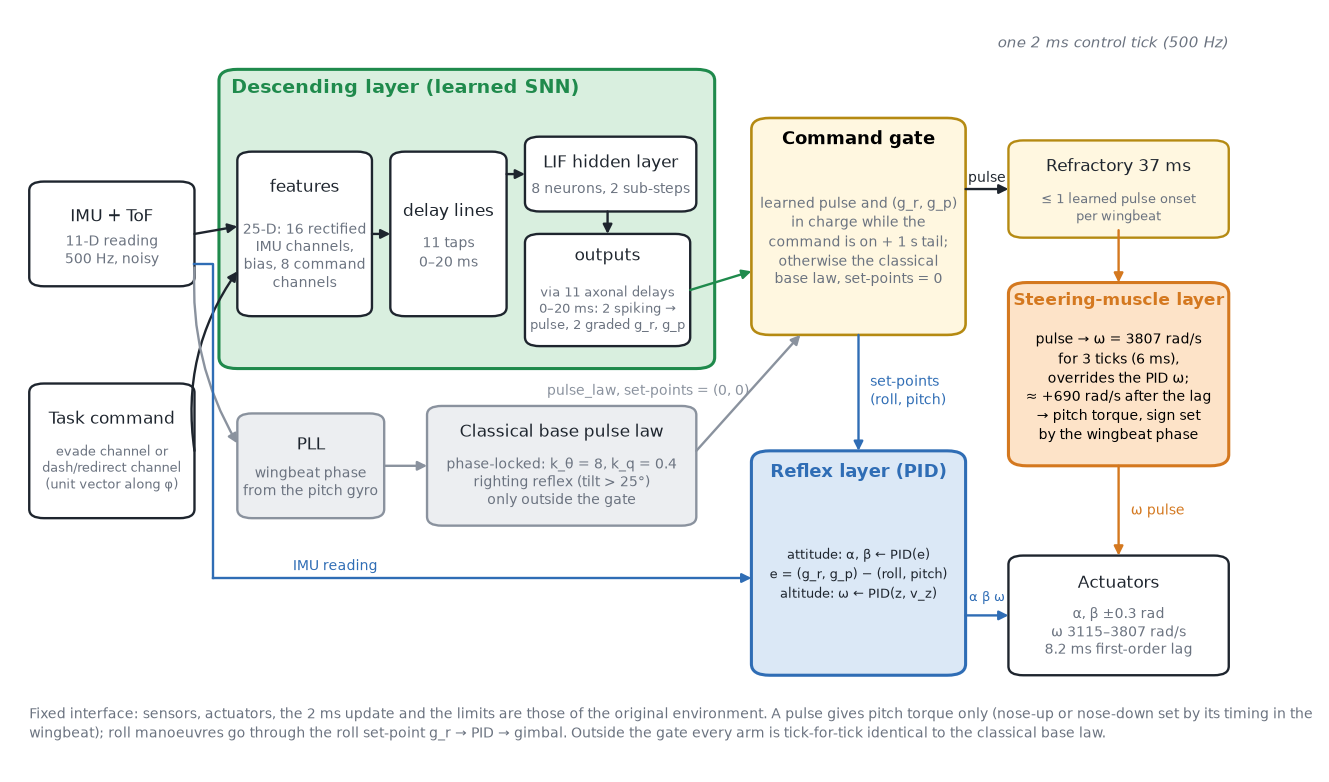
\includegraphics[width=\linewidth]{figs/fig_m1_architecture.png}\caption{\textbf{Fig. M1.} Three-layer controller in one 2 ms tick. The learned descending layer sees the 25-D rectified IMU/command features through 11 delay taps and emits motor-pulse spikes and graded roll/pitch set-points; the command gate hands control to it only while a manoeuvre is commanded (+1 s tail), otherwise the classical phase-locked base law acts. A pulse drives the motor to its maximum for 6 ms and produces a pitch torque whose sign is set by the wingbeat phase; roll goes through the set-point and the PID.}\label{fig:M1}\end{figure}
\begin{figure}[htbp]\centering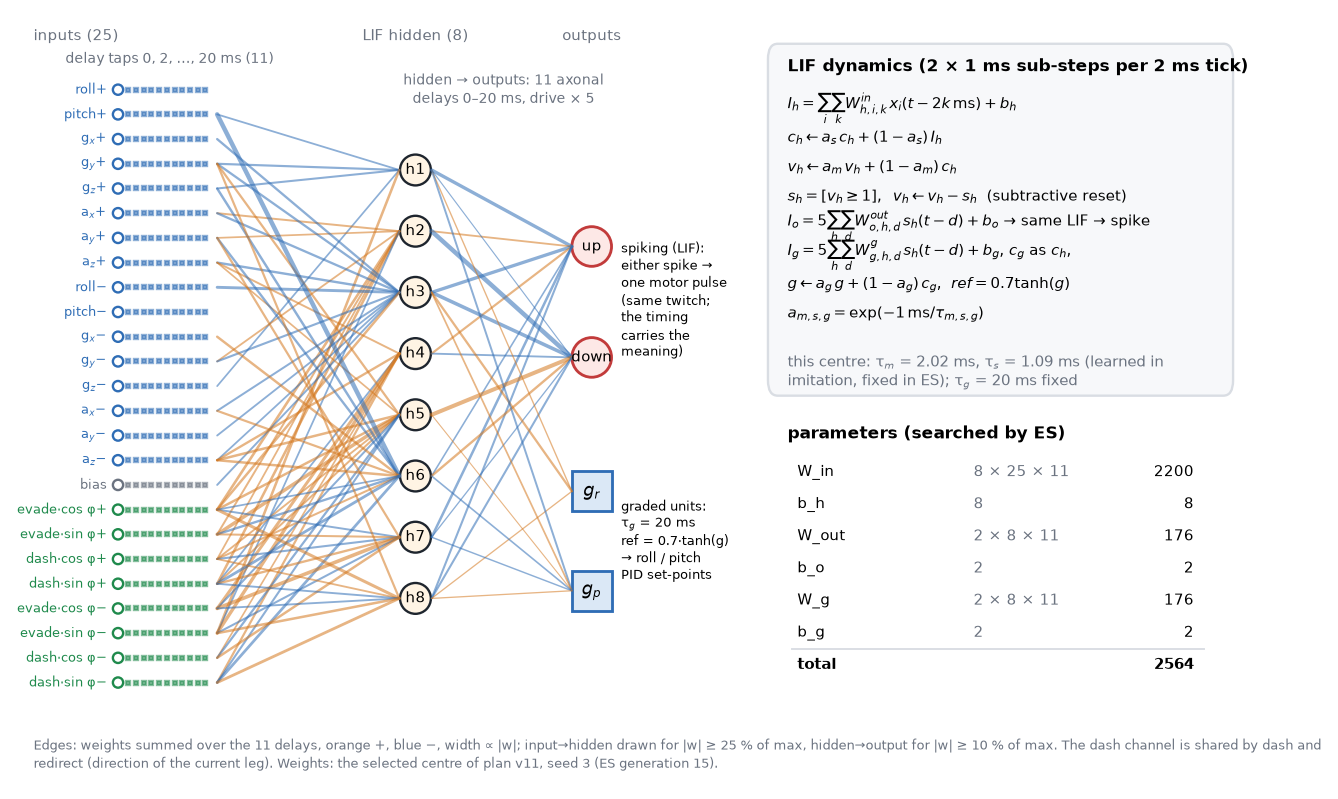
\includegraphics[width=\linewidth]{figs/fig_m2_snn.png}\caption{\textbf{Fig. M2.} The descending spiking network: 25 inputs $\times$ 11 delay taps $\rightarrow$ 8 LIF hidden neurons $\rightarrow$ two spiking outputs (either spike triggers the same twitch) and two graded units (set-points), with 11 axonal delays of 0--20 ms on the hidden spike trains. Edge widths are |weights| summed over delays for the selected plan-v11 centre of seed 3; right: update equations and the 2 564 ES-searched parameters (time constants learned in imitation, then frozen).}\label{fig:M2}\end{figure}
\begin{figure}[htbp]\centering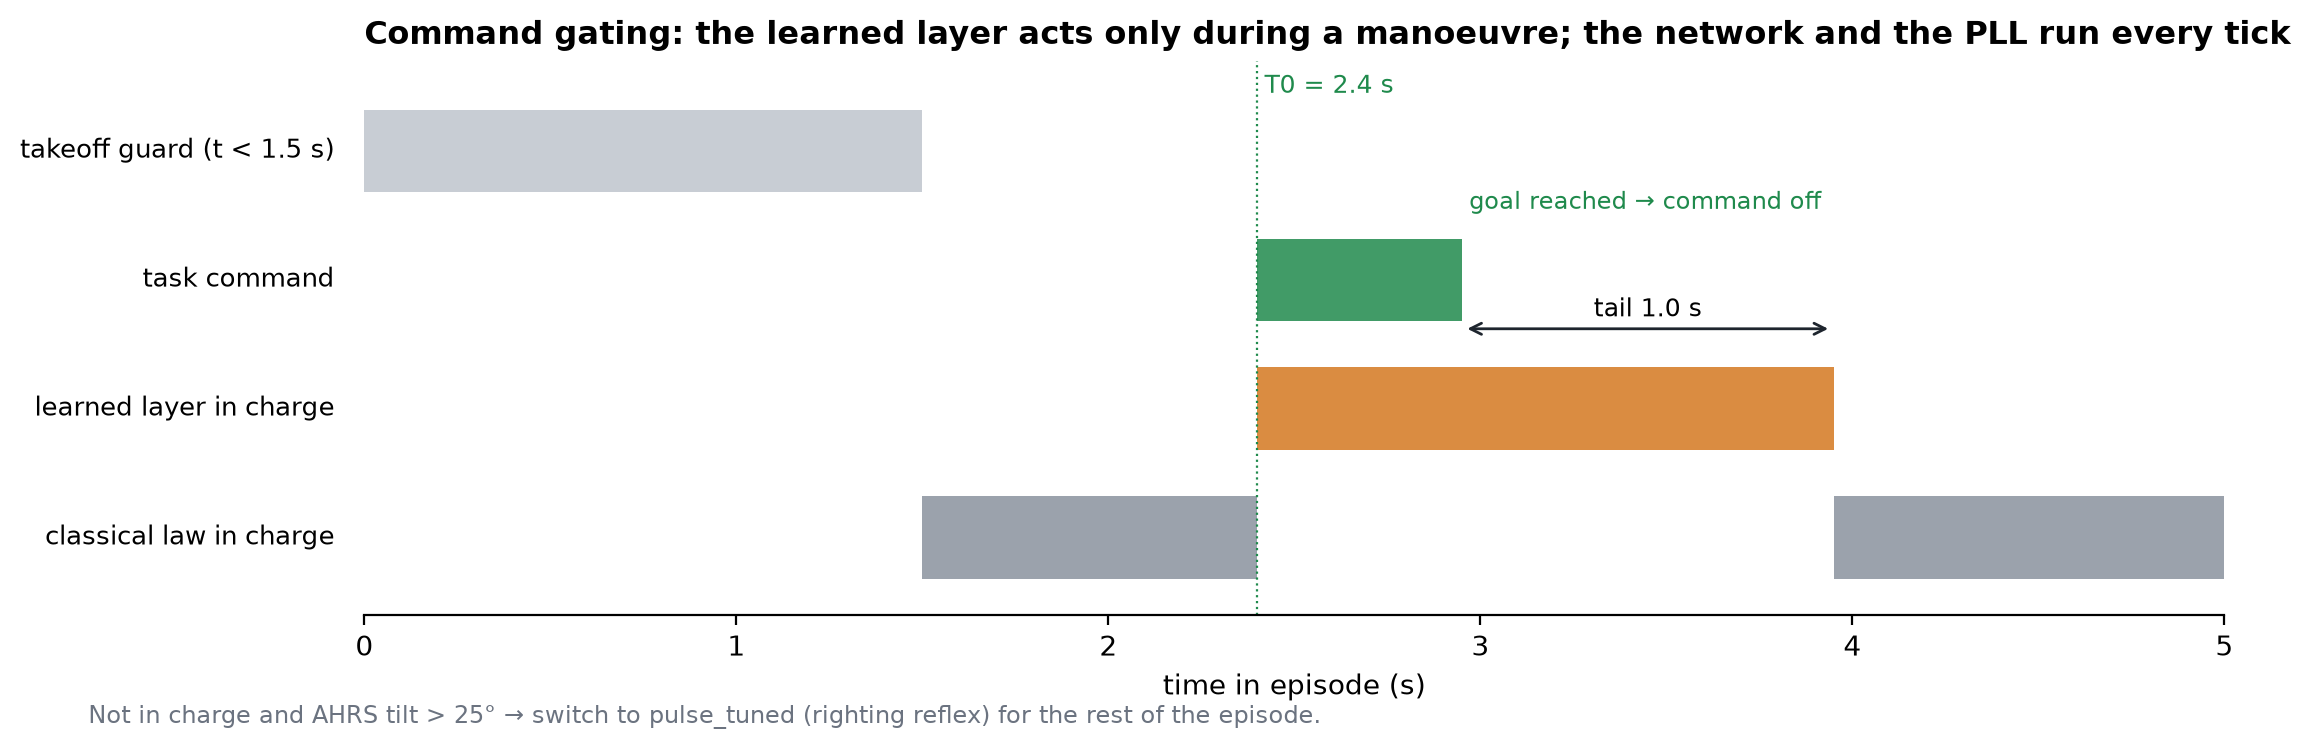
\includegraphics[width=\linewidth]{figs/fig_m3_gating.png}\caption{\textbf{Fig. M3.} Command gating in one dash/redirect episode (t0 = 2.4 s; evade draws t0 \textasciitilde{} U(2.2, 2.8) s; the time axis is truncated at 5 s of a 6.5 s episode). The learned layer may act only after the 1.5 s take-off guard, is in charge from the command onset until 1 s after the goal, and is otherwise replaced by the classical base law, so all arms fly identically before t0; outside the gate a sensed tilt above 25$^\circ$ switches to the righting law ("pulse\_tuned" in the figure).}\label{fig:M3}\end{figure}
\begin{figure}[htbp]\centering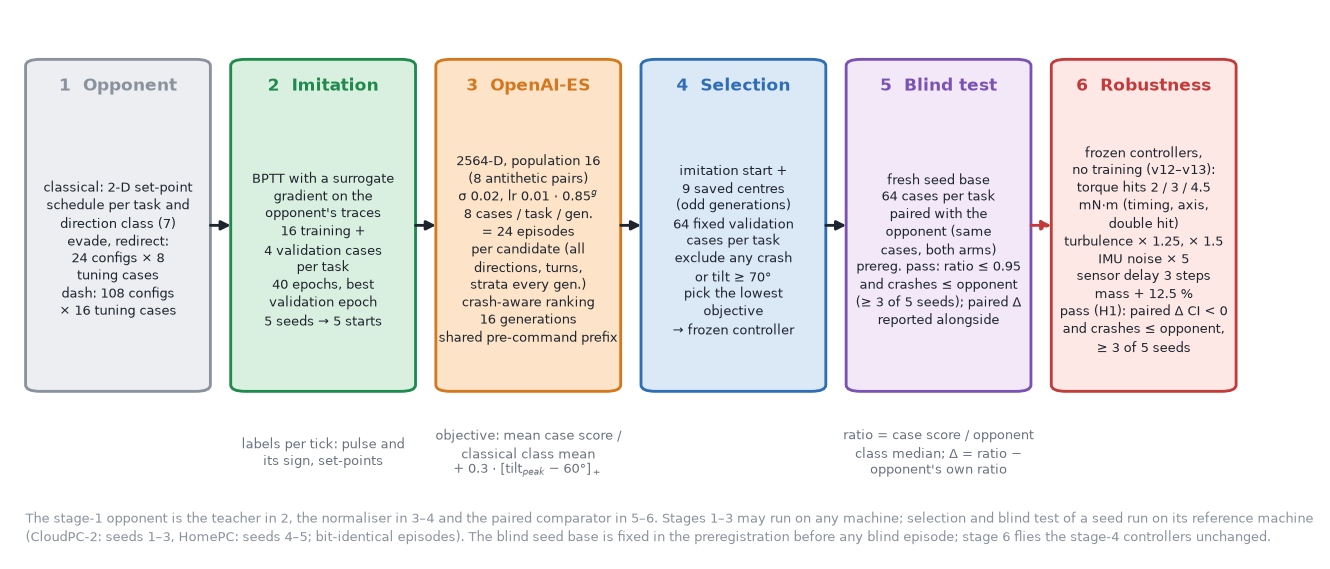
\includegraphics[width=\linewidth]{figs/fig_m4_pipeline.png}\caption{\textbf{Fig. M4.} Pipeline. The hand-tuned classical opponent (1) is the imitation teacher (2), the normaliser of the ES objective (3), the selection reference (4) and the paired comparator on every blind set (5, 6). Only the frozen output of stage 4 is evaluated blind; the robustness sets fly the same controllers unchanged.}\label{fig:M4}\end{figure}
\begin{figure}[htbp]\centering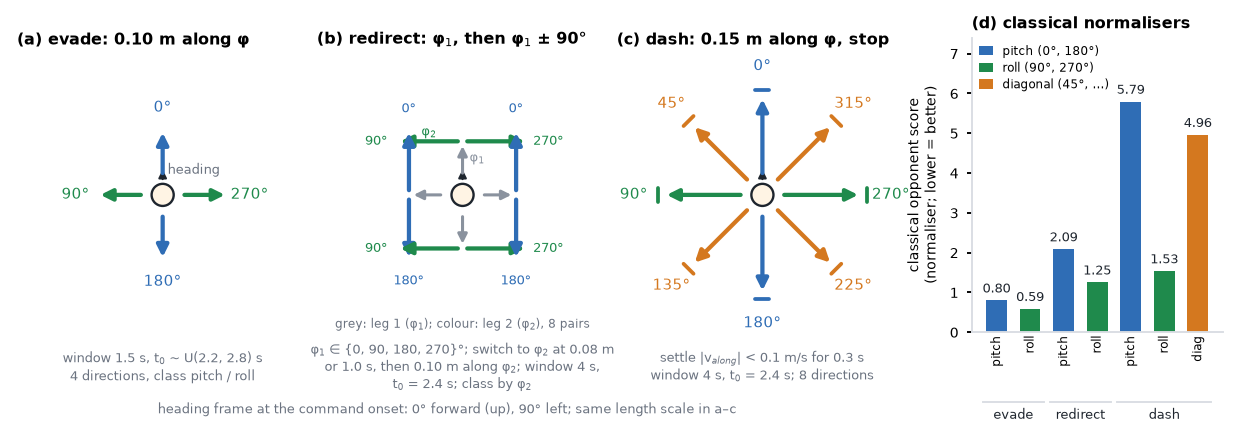
\includegraphics[width=\linewidth]{figs/fig_m5_tasks.png}\caption{\textbf{Fig. M5.} The three manoeuvres in the heading frame fixed at command onset (0$^\circ$ forward, 90$^\circ$ left): (a) evade 0.10 m in 4 directions, (b) redirect along $\varphi_1$ then $\varphi_2$ = $\varphi_1$ $\pm$ 90$^\circ$ (8 pairs, class by $\varphi_2$), (c) dash 0.15 m in 8 directions and settle; (d) the opponent's mean score per (task, class) on the 24 normalisation cases --- the ES normaliser; the blind-set ratio uses the opponent's class median on the blind cases.}\label{fig:M5}\end{figure}
\begin{figure}[htbp]\centering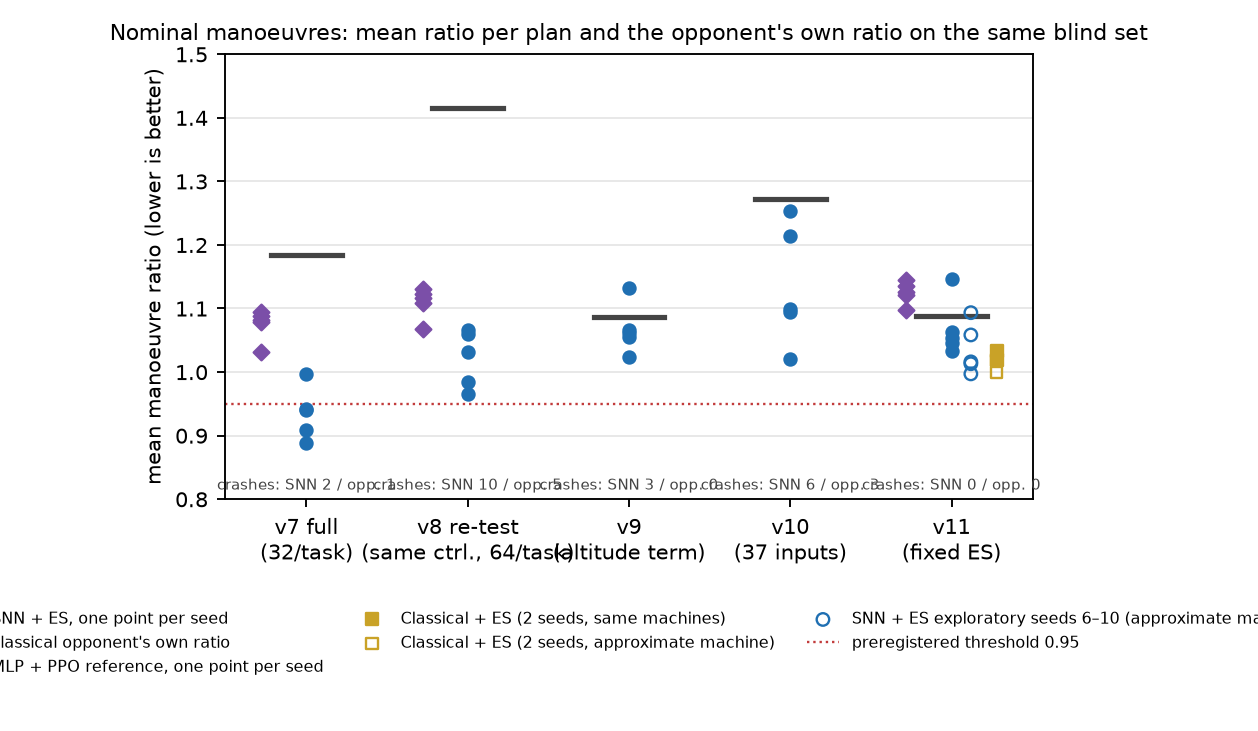
\includegraphics[width=\linewidth]{figs/fig_r0_nominal.png}\caption{\textbf{Fig. R0.} Mean manoeuvre ratio of SNN + ES on each plan's blind set (one point per seed; 64 cases per task, v7 full 32) against the threshold 0.95 and the classical opponent's own ratio on the same set (black), which exceeds 1 because scores are right-skewed. In v11, classical + ES (gold; open squares: approximate machine) does not reach 0.95 either. Crashes (SNN / opponent): v7 2/1, v8 10/5, v9 3/0, v10 6/3, v11 0/0. Hollow blue circles in the v11 column: the five exploratory SNN seeds 6--10 trained and tested on the approximate machine (their rows are under \texttt{artifacts/spike\_steer/googlecloud/}; not counted in any criterion).}\label{fig:R0}\end{figure}
\begin{figure}[htbp]\centering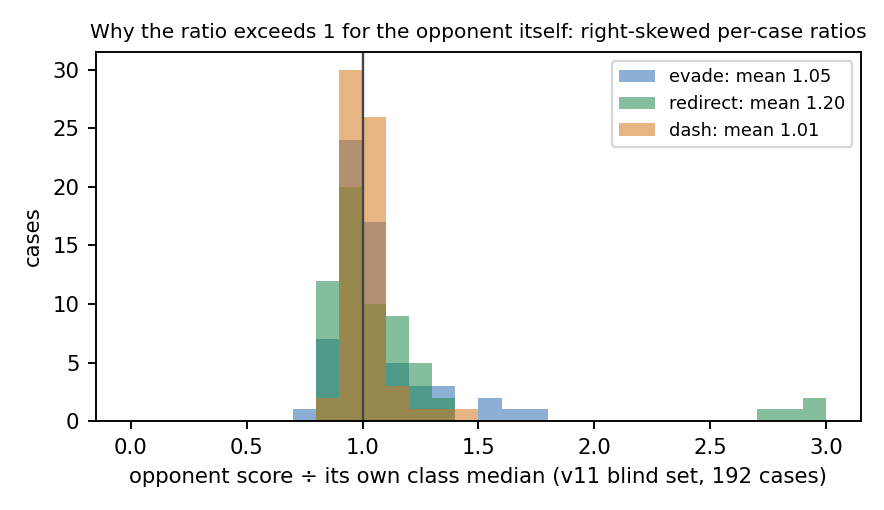
\includegraphics[width=\linewidth]{figs/fig_r0b_skew.png}\caption{\textbf{Fig. R0b.} Per-case ratio of the opponent's score to its own class median on the v11 blind set: medians near 1, means 1.01--1.20, a tail of slow or crashed cases.}\label{fig:R0b}\end{figure}
\begin{figure}[htbp]\centering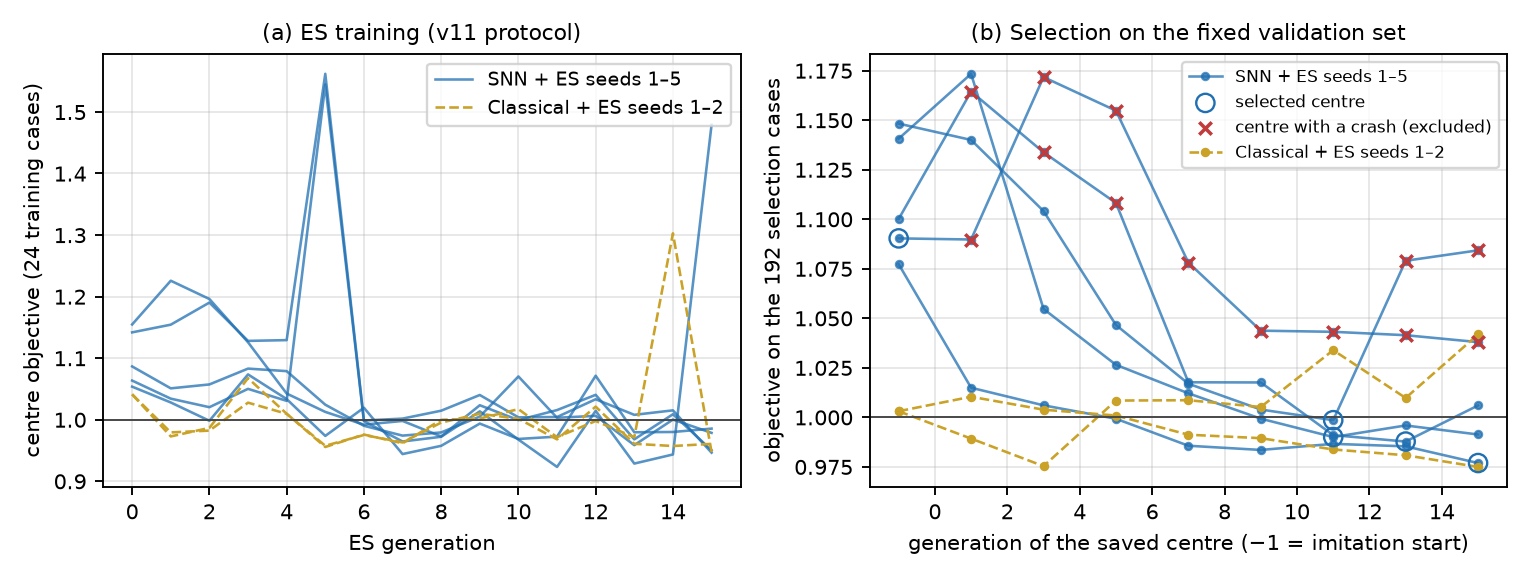
\includegraphics[width=\linewidth]{figs/fig_r1_training.png}\caption{\textbf{Fig. R1.} (a) Centre objective per ES generation on the 24-case batch (spikes --- SNN above 1.4, classical + ES 1.30 at generation 14 --- are generations in which the centre crashed on one batch case). (b) Objective of the nine saved centres on the fixed 192-case validation set; crosses = centres with a crash (excluded), circles = selected centre. Classical + ES (dashed) follows the same trajectory.}\label{fig:R1}\end{figure}
\begin{figure}[htbp]\centering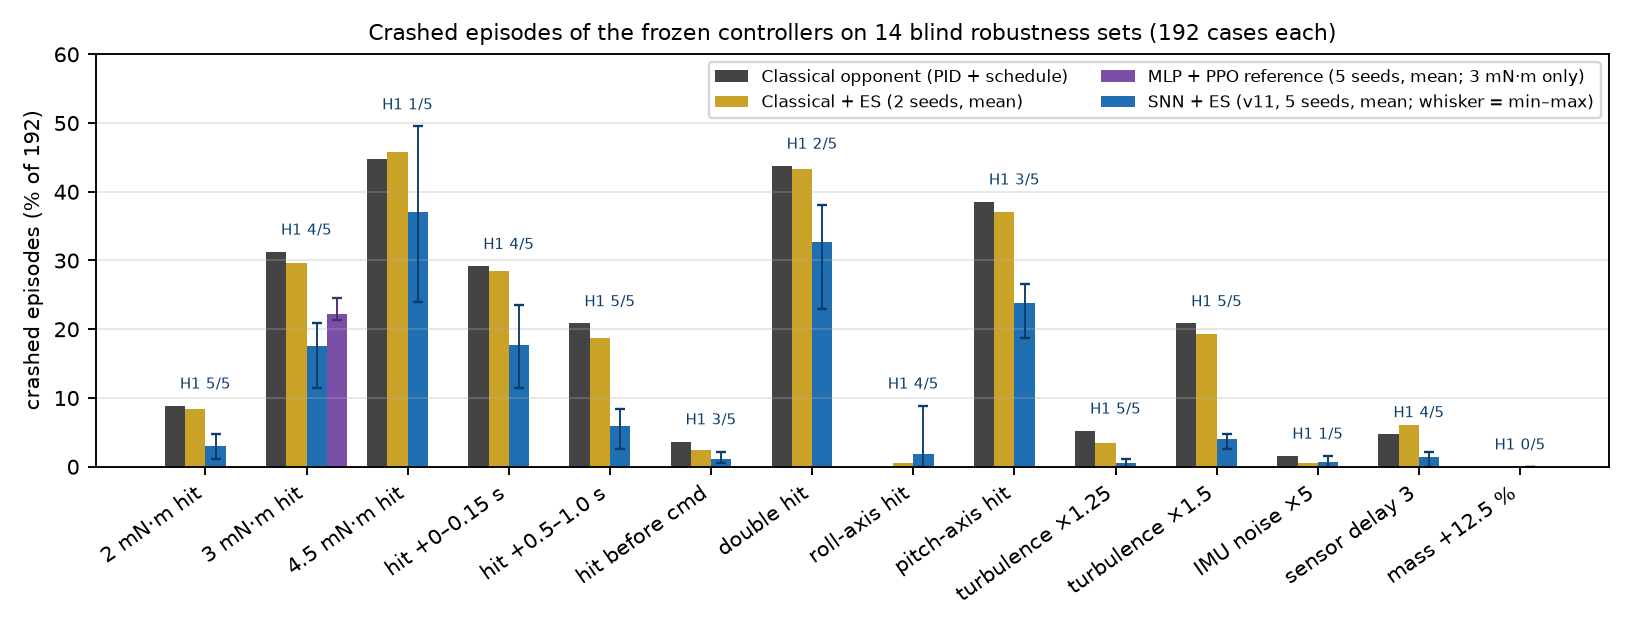
\includegraphics[width=\linewidth]{figs/fig_r2_crashes.png}\caption{\textbf{Fig. R2.} Crashed episodes (\% of 192) of the frozen controllers on 14 blind robustness sets ($\times$2/$\times$3 scaling omitted: every arm crashes > 90 \%). Dark grey: classical opponent; gold: classical + ES, mean of two seeds; blue: mean over five v11 seeds, whiskers = range; purple (3 mN$\cdot$m only): the MLP + PPO reference, mean of five seeds. "H1 n/5" = v11 seeds passing H1 relative to the opponent. Only the 3 mN$\cdot$m mid-manoeuvre hit is confirmatory.}\label{fig:R2}\end{figure}
\begin{figure}[htbp]\centering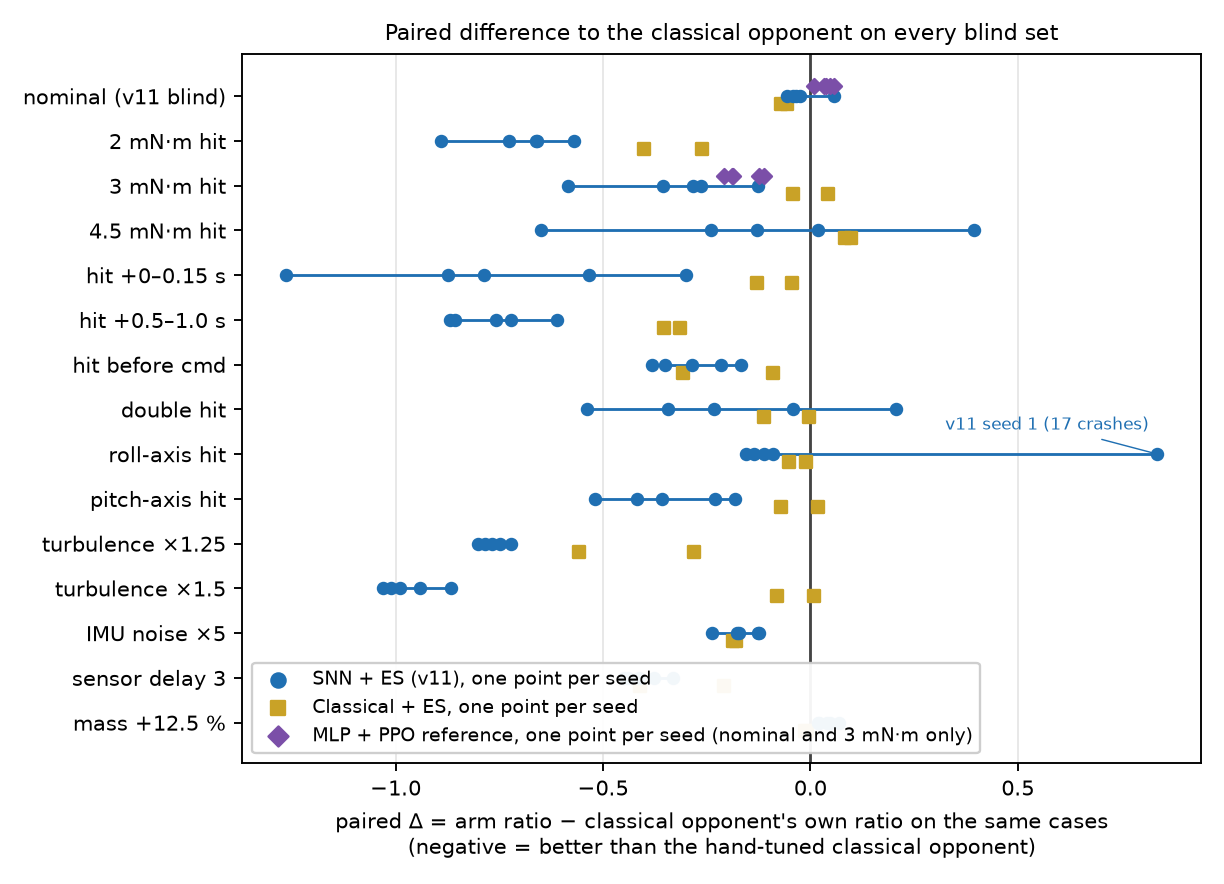
\includegraphics[width=\linewidth]{figs/fig_r3_paired_delta.png}\caption{\textbf{Fig. R3.} Paired $\Delta$ = arm ratio $-$ opponent's own ratio on identical cases, every blind set (negative = better). One point per seed; blue line = range over v11 seeds; squares = classical + ES; purple diamonds = MLP + PPO reference (nominal and 3 mN$\cdot$m rows only). Bootstrap intervals are not drawn; they are listed per seed in the per-scenario summaries (typical half-width 0.15--0.25 on the hit sets, 0.02--0.05 nominally). Outlier +0.84: v11 seed 1 on roll-axis hits (17 crashes where the opponent crashes 0 times).}\label{fig:R3}\end{figure}
\begin{figure}[htbp]\centering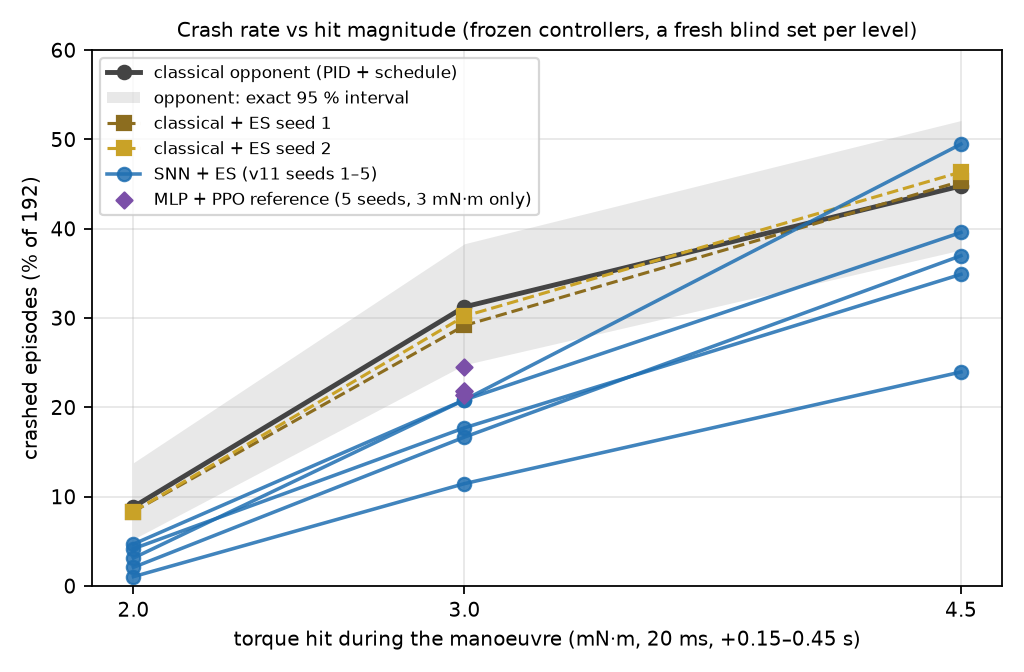
\includegraphics[width=\linewidth]{figs/fig_r4_dose_response.png}\caption{\textbf{Fig. R4.} Crash rate vs magnitude of a 20 ms torque hit 0.15--0.45 s into the manoeuvre (fresh set per level, 192 cases). Grey band: opponent's exact 95 \% interval; purple diamonds: the MLP + PPO reference at 3 mN$\cdot$m. Classical + ES tracks the opponent at every level; the learned layer's advantage over the opponent is largest at 2 mN$\cdot$m and vanishes for four of five seeds at 4.5 mN$\cdot$m.}\label{fig:R4}\end{figure}
\begin{figure}[htbp]\centering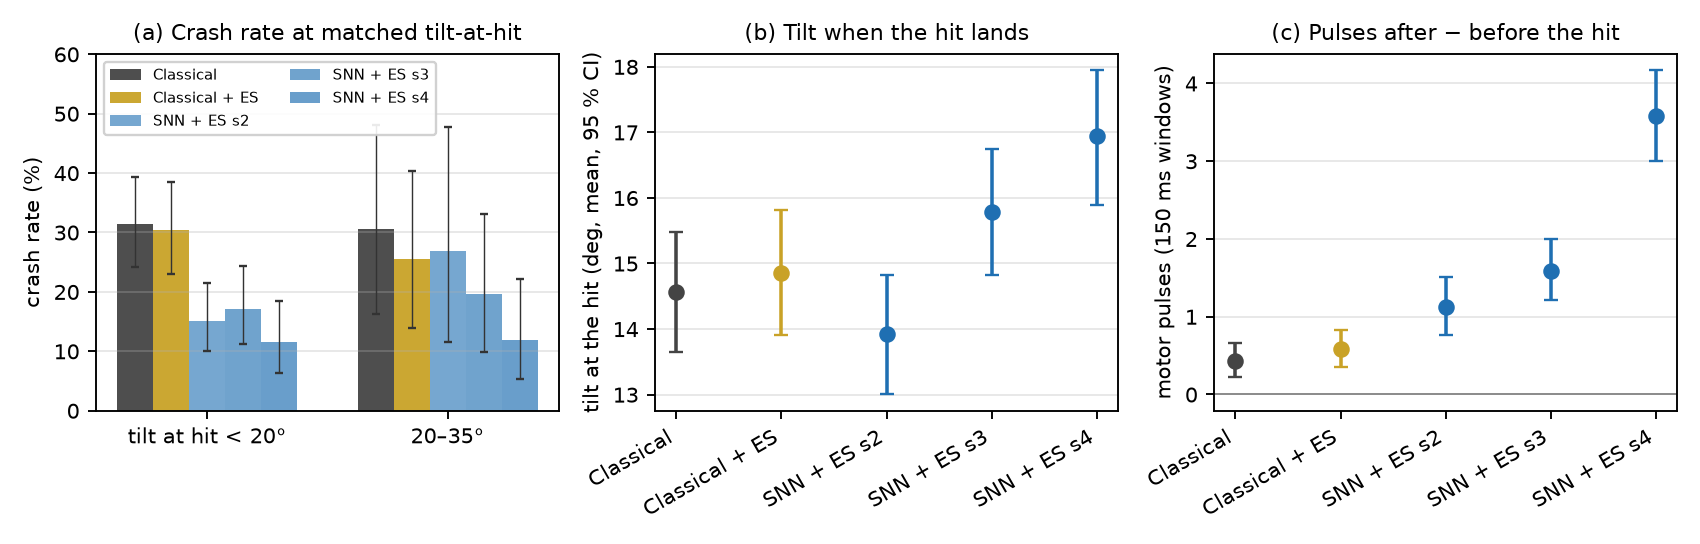
\includegraphics[width=\linewidth]{figs/fig_r5_mechanism.png}\caption{\textbf{Fig. R5.} Mechanism from the 192 primary cases re-flown with traces. (a) Crash rate at matched true tilt when the hit lands, with exact 95 \% intervals (n per bar: 156/36 opponent; 122--166 / 26--67 learned arms; the imitation start is in the data files); (b) mean tilt at the hit with 95 \% CI --- the learned arms do not fly at a smaller tilt; (c) motor pulses in the 150 ms after minus before the hit. The preregistered set-point measure was not met (projection on the induced tilt $\ge$ 0 for every arm).}\label{fig:R5}\end{figure}
\begin{figure}[htbp]\centering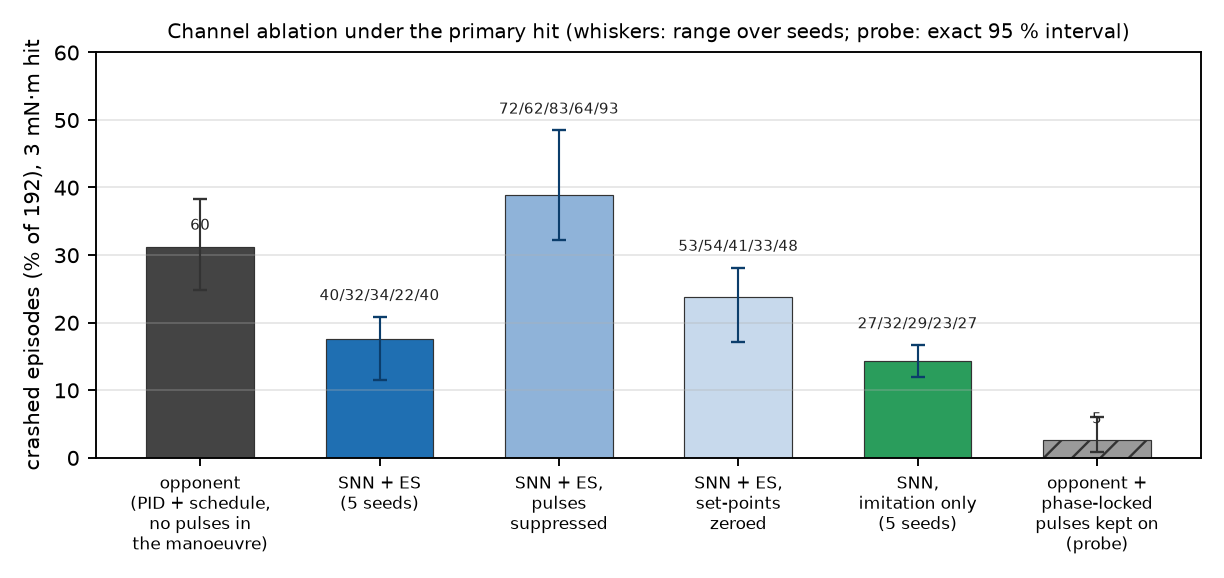
\includegraphics[width=\linewidth]{figs/fig_r5b_ablation.png}\caption{\textbf{Fig. R5b.} Channel ablation under the primary 3 mN$\cdot$m hit (crashes out of 192; whiskers: range over five seeds; numbers: per-seed counts). Suppressing the learned pulses while in charge removes the advantage over the opponent (62--93 vs 60); zeroing the set-points keeps most of it (33--54); the five imitation starts are as robust as the ES centres (23--32). Hatched: the mechanism probe --- the opponent with its own phase-locked hover pulse law kept on during the manoeuvre segments (5 crashes, exact 95 \% interval), which is not part of the classical manoeuvre design.}\label{fig:R5b}\end{figure}
\begin{figure}[htbp]\centering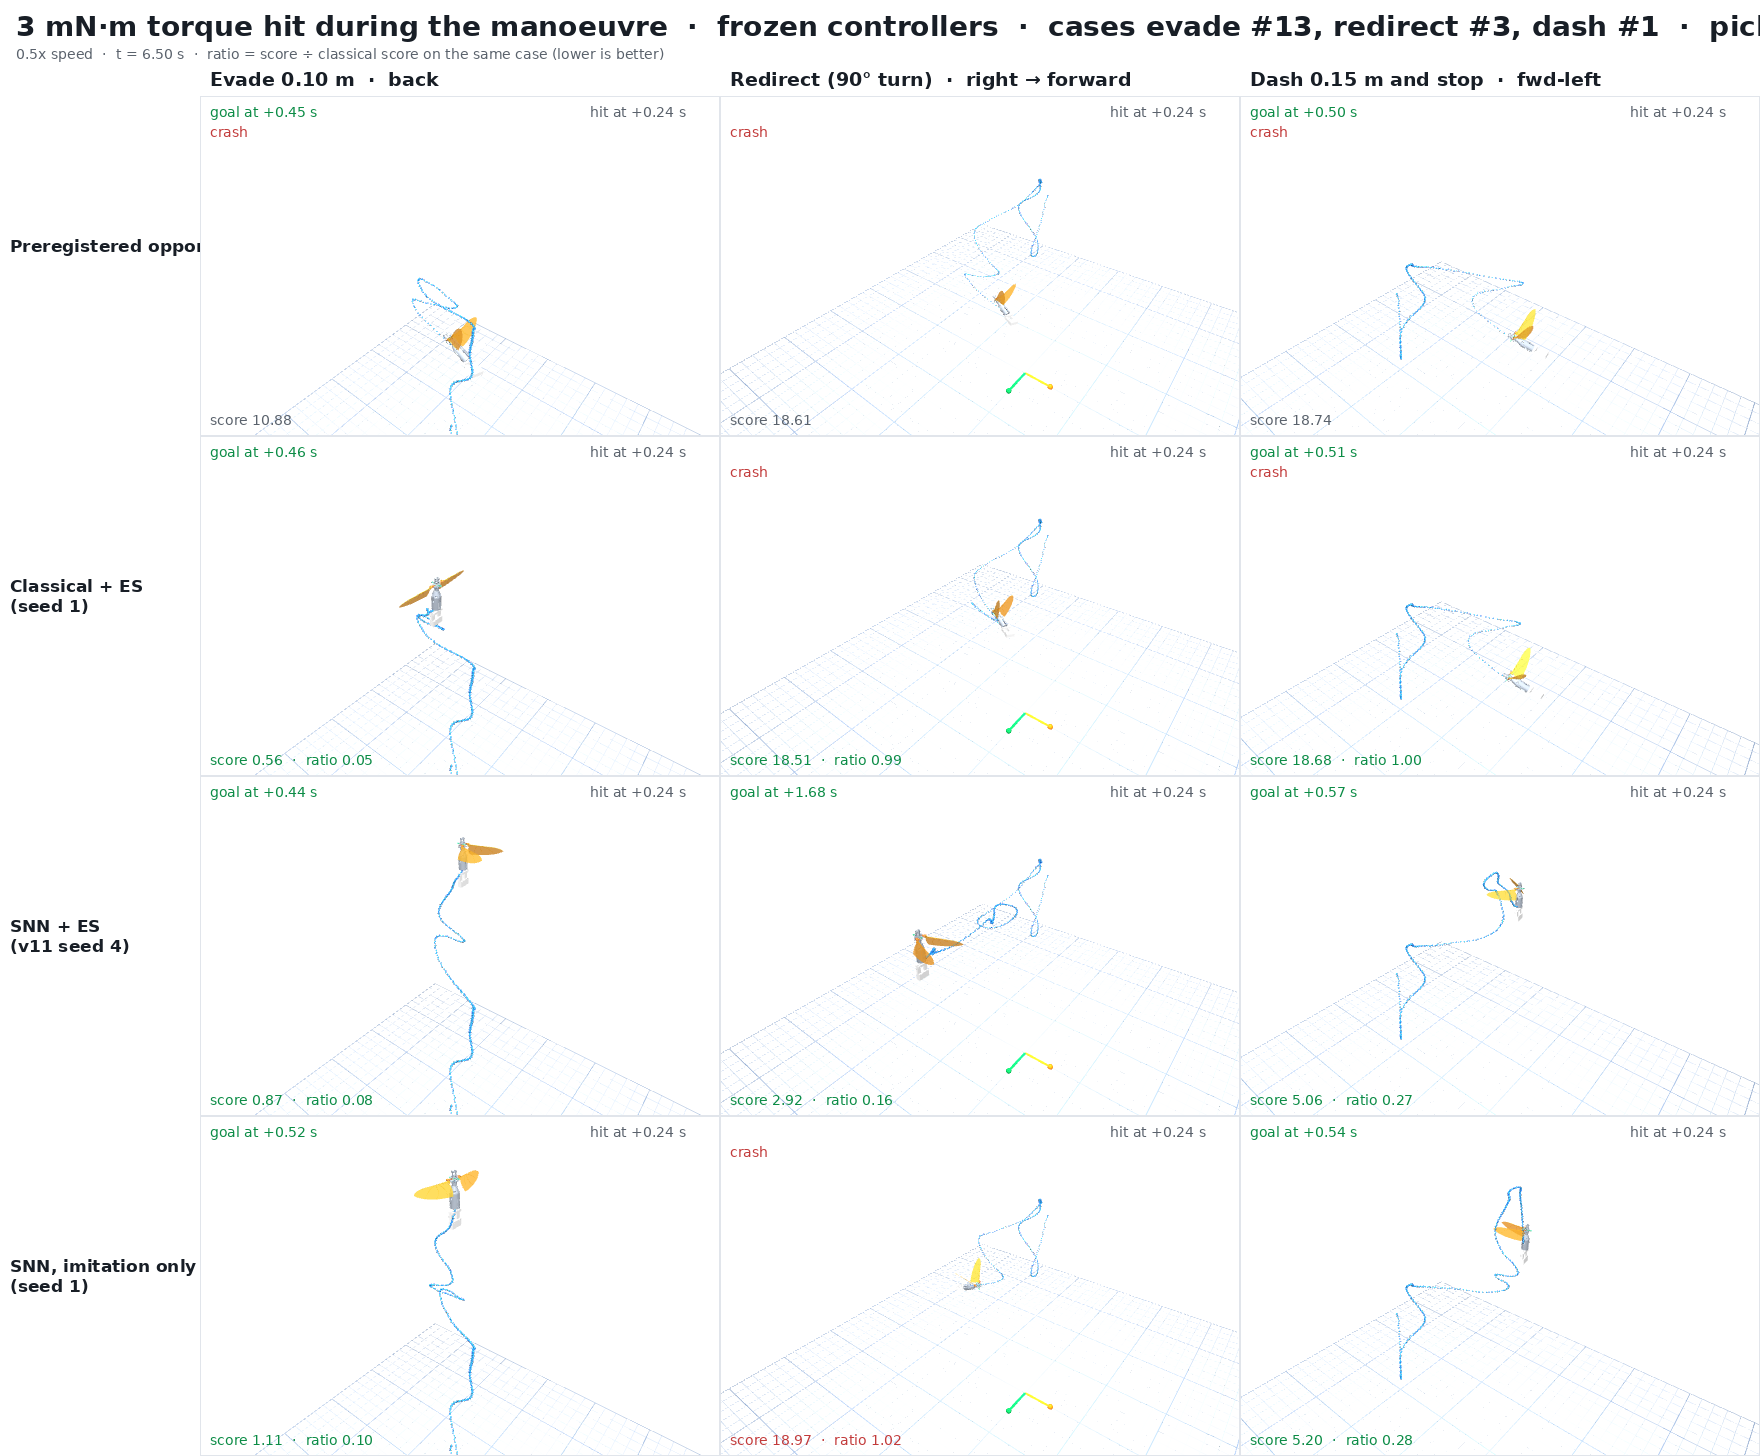
\includegraphics[width=\linewidth]{figs/fig_r6_kick_frame.png}\caption{\textbf{Fig. R6.} Illustrative final frames (t = 6.5 s, 0.5$\times$ playback of the video) of three primary-scenario cases, one per task, chosen because the classical opponent crashes and the v11 seed-4 centre completes the manoeuvre; the hit lands 0.24 s after the command. Rows: classical opponent, classical + ES (seed 1), SNN + ES (v11 seed 4), imitation start (seed 1). Not representative: on the full set the opponent crashes 60/192 and seed 4 22/192.}\label{fig:R6}\end{figure}
\end{document}
